% Options for packages loaded elsewhere
\PassOptionsToPackage{unicode}{hyperref}
\PassOptionsToPackage{hyphens}{url}
\PassOptionsToPackage{dvipsnames,svgnames,x11names}{xcolor}
\documentclass[
  10pt,
]{article}
\usepackage{xcolor}
\usepackage[a4paper,left=18mm,right=18mm,top=20mm,bottom=19mm]{geometry}
\usepackage{amsmath,amssymb}
\setcounter{secnumdepth}{-\maxdimen} % remove section numbering
\usepackage{iftex}
\ifPDFTeX
  \usepackage[T1]{fontenc}
  \usepackage[utf8]{inputenc}
  \usepackage{textcomp} % provide euro and other symbols
\else % if luatex or xetex
  \usepackage{unicode-math} % this also loads fontspec
  \defaultfontfeatures{Scale=MatchLowercase}
  \defaultfontfeatures[\rmfamily]{Ligatures=TeX,Scale=1}
\fi
\usepackage{lmodern}
\ifPDFTeX\else
  % xetex/luatex font selection
  \setmainfont[]{Times New Roman}
  \setsansfont[]{Arial}
  \setmonofont[]{Menlo}
\fi
% Use upquote if available, for straight quotes in verbatim environments
\IfFileExists{upquote.sty}{\usepackage{upquote}}{}
\IfFileExists{microtype.sty}{% use microtype if available
  \usepackage[]{microtype}
  \UseMicrotypeSet[protrusion]{basicmath} % disable protrusion for tt fonts
}{}
\makeatletter
\@ifundefined{KOMAClassName}{% if non-KOMA class
  \IfFileExists{parskip.sty}{%
    \usepackage{parskip}
  }{% else
    \setlength{\parindent}{0pt}
    \setlength{\parskip}{6pt plus 2pt minus 1pt}}
}{% if KOMA class
  \KOMAoptions{parskip=half}}
\makeatother
\usepackage{longtable,booktabs,array}
\usepackage{caption}
\captionsetup[table]{skip=6pt}
\newcounter{none} % for unnumbered tables
\usepackage{calc} % for calculating minipage widths
% Correct order of tables after \paragraph or \subparagraph
\usepackage{etoolbox}
\makeatletter
\patchcmd\longtable{\par}{\if@noskipsec\mbox{}\fi\par}{}{}
\makeatother
% Allow footnotes in longtable head/foot
\IfFileExists{footnotehyper.sty}{\usepackage{footnotehyper}}{\usepackage{footnote}}
\makesavenoteenv{longtable}
\usepackage{graphicx}
\makeatletter
\newsavebox\pandoc@box
\newcommand*\pandocbounded[1]{% scales image to fit in text height/width
  \sbox\pandoc@box{#1}%
  \Gscale@div\@tempa{\textheight}{\dimexpr\ht\pandoc@box+\dp\pandoc@box\relax}%
  \Gscale@div\@tempb{\linewidth}{\wd\pandoc@box}%
  \ifdim\@tempb\p@<\@tempa\p@\let\@tempa\@tempb\fi% select the smaller of both
  \ifdim\@tempa\p@<\p@\scalebox{\@tempa}{\usebox\pandoc@box}%
  \else\usebox{\pandoc@box}%
  \fi%
}
% Set default figure placement to htbp
\def\fps@figure{htbp}
\makeatother
\setlength{\emergencystretch}{3em} % prevent overfull lines
\providecommand{\tightlist}{%
  \setlength{\itemsep}{0pt}\setlength{\parskip}{0pt}}
\usepackage{fancyhdr}
\usepackage{xcolor}
\usepackage{titlesec}
\usepackage{float}
\definecolor{ink}{HTML}{19304A}
\definecolor{muted}{HTML}{526372}
\definecolor{rulegray}{HTML}{D5DDE4}
\pagestyle{fancy}
\fancyhf{}
\fancyhead[L]{\sffamily\scriptsize\color{muted} SPATIAL KDA / ARCHITECTURE AND CAUSAL TESTS}
\fancyhead[R]{\sffamily\scriptsize\color{muted} 23 SEPTEMBER 2026}
\fancyfoot[L]{\sffamily\scriptsize\color{muted} Measured architecture and metrics; proposed interventions}
\fancyfoot[R]{\sffamily\scriptsize\thepage}
\renewcommand{\headrulewidth}{0.3pt}
\renewcommand{\footrulewidth}{0pt}
\setlength{\headheight}{14pt}
\setlength{\headsep}{13pt}
\setlength{\footskip}{20pt}
\titleformat{\section}{\sffamily\Large\bfseries\color{ink}}{}{0pt}{}
\titleformat{\subsection}{\sffamily\normalsize\bfseries\color{ink}}{}{0pt}{}
\titlespacing*{\section}{0pt}{0pt}{10pt}
\titlespacing*{\subsection}{0pt}{9pt}{5pt}
\setlength{\parskip}{5pt}
\setlength{\parindent}{0pt}
\setlength{\emergencystretch}{2em}
\setlength{\tabcolsep}{4pt}
\renewcommand{\arraystretch}{1.13}
\floatplacement{figure}{H}
\AtBeginDocument{\hypersetup{colorlinks=true,linkcolor=ink,urlcolor=ink}}
\usepackage{bookmark}
\IfFileExists{xurl.sty}{\usepackage{xurl}}{} % add URL line breaks if available
\urlstyle{same}
% fallback for those not using the hyperref driver hyperxmp:
\makeatletter
\@ifundefined{xmpquote}{\newcommand{\xmpquote}[1]{#1}}{}
\makeatother
\hypersetup{
  colorlinks=true,
  linkcolor={Maroon},
  filecolor={Maroon},
  citecolor={Blue},
  urlcolor={Blue},
  pdfcreator={LaTeX via pandoc}}

\author{}
\date{}

\begin{document}

\section{1. Spatial KDA memory: architecture and causal
tests}\label{spatial-kda-memory-architecture-and-causal-tests}

\textbf{Technical research note · 23 September 2026}\\
\textbf{Scope:} the current fresh-weight, 13-task joint learner,
continued from step 715. Architecture is implemented; behavioral metrics
are measured; all microstimulation protocols below are proposals, not
completed interventions.

\subsection{Executive assessment}\label{executive-assessment}

The model combines a convolutional visual hierarchy with three spatial
associative memories and a final global gated recurrent unit (GRU).
Memory therefore affects visual processing at multiple resolutions,
rather than existing only behind the encoder. Each of thirteen tasks has
a separate linear classifier, but all visual processing, spatial
memories and the global recurrent summary are shared. There is no
explicit object-slot memory, no top-down GRU-to-encoder feedback, and no
spatial softmax that competitively divides a fixed attention budget
among scene locations.

\begin{figure}
\centering
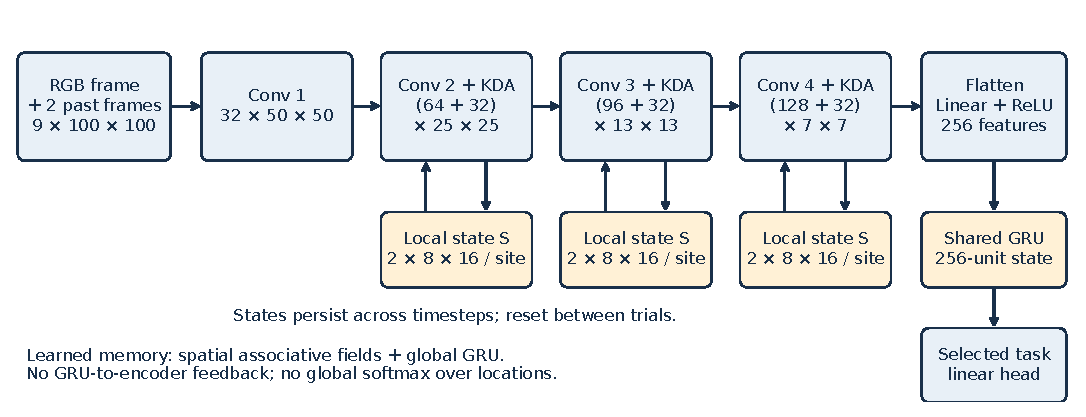
\includegraphics[width=1\linewidth,height=\textheight,keepaspectratio,alt={Implemented computation. Gold boxes are recurrent state, not separately trained modules. Every learned component remains trainable.}]{architecture.pdf}
\caption{Implemented computation. Gold boxes are recurrent state, not
separately trained modules. Every learned component remains trainable.}
\end{figure}

The completed short run acquired contrast, chromatic increments and
natural-image spectral-detail discrimination, but not robust spatial
selection, motion accumulation, binding or scene recognition. The
ongoing continuation has substantially improved spatial-frequency
discrimination and produced preliminary score-level motion/orientation
signals. Those observations support continued acquisition; they do not
yet establish a competent attentional observer or explain where failures
arise.

Morgan, Albanna and Herman's recurrent vision transformer provides a
useful \textbf{functional comparison}, not an interchangeable mechanism.
Their artificial-bias experiment forces spatial allocation toward a
location and measures change reports and response timing; our KDA
exposes signed associative matrices and emitted features, not the same
allocation variable.{[}1{]} A local perturbation can test whether a
representation causally influences behavior. It cannot, simply by being
called ``microstimulation,'' establish correspondence to electrical
current injection, a particular brain area, or the paper's exact
manipulation.

\textbf{Main recommendation.} First establish appropriate task
competence and sham equivalence. Then perturb a calibrated local
representation at matched sites and epochs, measuring psychometric
changes, false reports, sensitivity and criterion. Treat enhancement,
interference, disruption and null effects as distinct possible outcomes.
Do not assume that increasing local activity should improve performance
or reproduce the paper's cue-versus-change timing effect.

\textbf{Evidence boundary.} This report describes the current joint
lineage, not the historical orientation-only KDA trained with a
different curriculum. Earlier successes are neither its initialization
nor evidence that this learner has acquired the same mechanisms. No
stimulation, inhibition, new calibration extraction or additional model
evaluation was performed to write this document.

\newpage

\section{2. The implemented visual and memory
hierarchy}\label{the-implemented-visual-and-memory-hierarchy}

The input is a float32 tensor
\(X\in[0,1]^{B\times T\times3\times100\times100}\). A batch contains one
task and one condition, avoiding artificial sequence padding across
different conditions. The model subtracts \(0.5\) and constructs a
causal channel stack \([X_{t-2},X_{t-1},X_t]\). Unavailable history is
zero in centered coordinates. This is explicit short-term sensory
access, not a learned memory or an additional presented observation:
two-frame tasks still contain exactly two observed frames. {[}C1, C3{]}

\subsection{Spatial processing}\label{spatial-processing}

Each encoder block is a stride-two convolution followed by eight-group
GroupNorm and ReLU. The first kernel is \(5\times5\); the remaining
kernels are \(3\times3\), with padding preserving the specified
downsampling convention. After each of the last three blocks, a learned
\(1\times1\) convolution projects current features to 32 channels for a
distinct KDA module. Its 32-channel emission is concatenated with the
block's visual output.

{\def\LTcaptype{none} % do not increment counter
\begin{longtable}[]{@{}
  >{\raggedright\arraybackslash}p{(\linewidth - 6\tabcolsep) * \real{0.2308}}
  >{\raggedleft\arraybackslash}p{(\linewidth - 6\tabcolsep) * \real{0.3077}}
  >{\raggedright\arraybackslash}p{(\linewidth - 6\tabcolsep) * \real{0.2308}}
  >{\raggedright\arraybackslash}p{(\linewidth - 6\tabcolsep) * \real{0.2308}}@{}}
\toprule\noalign{}
\begin{minipage}[b]{\linewidth}\raggedright
Stage
\end{minipage} & \begin{minipage}[b]{\linewidth}\raggedleft
Block input channels
\end{minipage} & \begin{minipage}[b]{\linewidth}\raggedright
Visual output
\end{minipage} & \begin{minipage}[b]{\linewidth}\raggedright
Output after memory concatenation
\end{minipage} \\
\midrule\noalign{}
\endhead
\bottomrule\noalign{}
\endlastfoot
Conv 1 & 9 & \(32\times50\times50\) & No KDA at this stage \\
Conv 2 & 32 & \(64\times25\times25\) & \(96\times25\times25\) \\
Conv 3 & 96 & \(96\times13\times13\) & \(128\times13\times13\) \\
Conv 4 & 128 & \(128\times7\times7\) & \(160\times7\times7\) \\
\end{longtable}
}

The final concatenated map is flattened and passed through a learned
linear projection and ReLU to 256 features. The configured optional
feature normalization is the identity, not LayerNorm. A single-layer,
256-unit GRU receives the feature sequence, and the task's linear head
reads its final hidden state. No intermediate task decision is emitted
by the deployed model. {[}C1{]}

\subsection{What is stored, and where?}\label{what-is-stored-and-where}

For each resolution \(s\), spatial site \(p\) and associative head
\(h\), KDA stores\\
\[
S_{t,p,h}^{(s)}\in\mathbb{R}^{8\times16},\qquad h\in\{1,2\}.
\]\\
The full state tensor is
\(B\times H_s\times W_s\times2\times8\times16\). It is a learned
key-to-value association at each feature location---not an eight-object
store, sixteen named stimulus attributes or a biological synaptic count.
Memory matrices and values can be signed. Each scale has its own
trainable parameters and its own state. The two heads' emissions form
the 32-channel readout field. {[}C2{]}

Spatial coordinates are preserved in KDA, but a feature-map site is not
an isolated image pixel or one experimental stimulus. Overlapping
receptive fields, successive downsampling and convolutional mixing
matter. GroupNorm also uses spatial statistics within channel groups, so
the consequences of a localized feature intervention need not remain
strictly local. Masks must be defined in scene coordinates, mapped to
each scale, and verified against actual propagation.

The final GRU supplies another recurrent route. A cue could influence a
later decision through local KDA, global GRU, their interaction or
residual stacked input. The existence of spatial state does not prove
that behavior uses it, and a global memory reset would confound these
routes rather than isolate a local mechanism.

\textbf{Verified size.} There are \textbf{2,750,324 trainable
parameters}: encoder blocks 256,992; projections 9,312; KDA modules
74,262; dense feature projection 2,007,296; GRU 394,752; task heads
7,710. KDA holds \textbf{215,808 state scalars per example} (160,000 /
43,264 / 12,544 across scales), or 863,232 fp32 bytes. Including the GRU
gives 216,064 recurrent scalars, excluding the raw-frame stack, BPTT
intermediates and optimizer storage. These are activation counts, not
additional learned parameters. {[}R3{]}

\newpage

\section{3. KDA equations, retention and the readout
bottleneck}\label{kda-equations-retention-and-the-readout-bottleneck}

At a fixed scale/site/head, suppress those indices and let
\(u_t\in\mathbb{R}^{32}\) denote projected current features. A learned
\(3\times3\) convolution produces packed query, key, value and gate
vectors. Each head uses dimensions \(8+8+16+8+1\). Queries and keys are
L2-normalized with numerical epsilon \(10^{-6}\); values are
unconstrained. Elementwise sigmoid gives row-retention
\(\boldsymbol\alpha_t\in(0,1)^8\) and scalar write strength
\(\beta_t\in(0,1)\). {[}C2{]}

The implemented update is\\
\[
\bar S_t=D_{\boldsymbol\alpha_t}S_{t-1},\qquad
 e_t=v_t-\bar S_t^\top k_t,
\]\\
\[
 S_t=\bar S_t+\beta_t k_t e_t^\top,\qquad
 o_t=S_t^\top q_t.
\]\\
The two 16-dimensional outputs are concatenated and transformed by a
learned \(1\times1\) convolution. That emitted field is joined to the
current visual features before the next processing stage. The output
projection has a bias; the recurrent matrix is not identical to the
emitted feature field.

\subsection{Interpretation and limited stability
claim}\label{interpretation-and-limited-stability-claim}

This is a \textbf{prediction-error write}, not an unweighted running
sum. The current key first retrieves a prediction; the update corrects
its error toward the incoming value. Retention can forget old
associations, and nonorthogonal keys can interfere. The same learned
rule can implement useful persistence, selective replacement or an
unhelpful recency bias depending on learned representations and gates.

Equivalently,\\
\[
 S_t=(I-\beta_t k_t k_t^\top)D_{\boldsymbol\alpha_t}S_{t-1}
       +\beta_t k_t v_t^\top.
\]\\
For a fixed gate/key sequence with \(\|k_t\|_2\leq1\), the homogeneous
state-transition norm is bounded by \(\max_j\alpha_{t,j}\leq1\). This
follows from the eigenvalues of the rank-one correction and diagonal
retention. It is a conditional algebraic bound, \textbf{not} proof of
stable gradients or bounded activity in the entire learned recurrent
network: values are unbounded, gates are input-dependent, upstream
features depend on earlier memory emissions, and the global GRU forms an
additional route. No forgetting time constant is inferred from this
inequality.

Gate weights were initialized so retention starts at \(0.9\) and write
strength at \(0.5\), initially independent of input. They remain
trainable; those initialization values are not the trained retention
law. Numerical checks reject nonfinite loss, gradients or parameters.
This run does not clip gradients. {[}C2, C4{]}

\subsection{Decision route and temporal
interpretation}\label{decision-route-and-temporal-interpretation}

All spatial emissions must pass through a dense 256-dimensional
projection and the shared GRU before reaching a task head. The
projection preserves the possibility of location-specific weights
through flattening, but creates a substantial compression relative to
the full spatial state. A failed decision could therefore reflect poor
encoding, weak retention, interference, inadequate comparison, or
ineffective use of information that remains stored. Scores alone do not
identify which explanation applies.

The GRU and KDA states reset at each trial; only trained parameters
persist between trials. During a nominal blank, the frame stack can
still contain a sample for the first two updates. A retention
intervention must distinguish those residual sensory-access frames from
genuinely stimulus-free processing. The ring task's final stack contains
both sample frames: success there alone would not establish blank-delay
memory. Frame counts are not biological milliseconds without a
renderer-defined clock.

\newpage

\section{4. Task semantics and optimization
exposure}\label{task-semantics-and-optimization-exposure}

The suite has thirteen task heads and 35 primary conditions. Task
identity selects the head externally; the network is not learning which
task the experimenter requested. Only images enter the sensory/recurrent
path. Cue positions, renderer phases, labels, actual angles and image
identities remain analysis metadata. {[}C3{]}

{\def\LTcaptype{none} % do not increment counter
\begin{longtable}[]{@{}
  >{\raggedright\arraybackslash}p{(\linewidth - 4\tabcolsep) * \real{0.3000}}
  >{\raggedright\arraybackslash}p{(\linewidth - 4\tabcolsep) * \real{0.3000}}
  >{\raggedleft\arraybackslash}p{(\linewidth - 4\tabcolsep) * \real{0.4000}}@{}}
\toprule\noalign{}
\begin{minipage}[b]{\linewidth}\raggedright
Family
\end{minipage} & \begin{minipage}[b]{\linewidth}\raggedright
Required report
\end{minipage} & \begin{minipage}[b]{\linewidth}\raggedleft
Primary cells
\end{minipage} \\
\midrule\noalign{}
\endhead
\bottomrule\noalign{}
\endlastfoot
Motion direction & Cardinal direction between two dot frames & 1 \\
Signed orientation & Sign of two-frame axial-angle change & 1 \\
Contrast & Which frame has greater contrast? & 1 \\
Spatial frequency & Which frame has higher frequency? & 1 \\
Chromatic increment & Which frame contains the defined colour increment?
& 1 \\
Contour grouping & Which frame contains the aligned contour? & 1 \\
Natural spectral detail & Which image has greater high-frequency detail?
& 1 \\
Ring orientation & Sign of change at ring-cued Gabor & 1 \\
Cued orientation & Target change matches spatial +/− instruction & 4 \\
Cued motion duration & Most frequent direction at the cued patch & 4 \\
Krauzlis change & Target change, versus foil change or catch & 3 \\
Spatial binding & Queried location participated in an orientation swap &
4 \\
Scene recognition & Probe is an exact member of the study set & 12 \\
\end{longtable}
}

The seven sensory tasks have two presented frames. Ring orientation has
cue, two sample frames and probe, with no inserted blanks. Cued
orientation, duration and binding use inserted delays
\(D\in\{0,4,12,24\}\). Binding uses a retrospective query, not an
encoding precue. Krauzlis conditions \(B\in\{12,20,28\}\) vary baseline
motion transitions, not memory delays. Recognition combines study
lengths \(N\in\{0,4,12,24\}\) with three, four or five repetitions of
the same probe. Repeated frames are not independent episodes. {[}C3{]}

\subsection{Why these distinctions matter for causal
comparison}\label{why-these-distinctions-matter-for-causal-comparison}

The signed cued-orientation task is not an unrestricted ``any change''
detector. An opposite-sign target rotation is a negative report, even
though a physical change occurred. Binding negatives still contain a
foil swap. Krauzlis foil changes are deliberately negative. By contrast,
a real uncued change is a valid detection event in the reference paper's
any-change task.{[}1{]} An intervention that increases reporting of
uncued changes can therefore improve one task while violating another;
calling both outcomes an attentional benefit would be misleading.

\subsection{Training contract}\label{training-contract}

All components train jointly from a fresh initial model, using mean
cross-entropy and Adam at \(10^{-4}\) with one parameter group, zero
weight decay, no clipping, fp32 and full-sequence BPTT. Effective batch
size is 32 via microbatches of four. A shuffled cycle contains one
update per task; condition queues cycle within each task. A task head
receives gradients only on that task's updates, while shared processing
receives all task losses. {[}C4{]}

The completed run used 715 updates, 22,880 episodes and 55 task-specific
updates per head. The current eight-hour continuation preserves its
weights, Adam state, streams and RNG, targeting 2,145 additional
updates: 2,860 cumulative updates and 91,520 episodes if completed. The
old horizon is not a plateau criterion. Training allocation, stimuli and
architecture did not change during this continuation;
checkpoint-selection policy changed prospectively, as discussed on page
6.

\newpage

\section{5. Preliminary behavioral
metrics}\label{preliminary-behavioral-metrics}

\textbf{Evidence frozen at 06:48:15 UTC, 23 September 2026.} The running
model had reached step 2647 / 84,704 episodes; its latest completed
validation was step 2314. The table contrasts completed step-715 tests
with that validation---not paired draws or the unmeasured performance of
step 2647. V3 final tests were pending at the cutoff. BA averages
eligible conditions equally within each task. {[}R1--R3{]}

{\def\LTcaptype{none} % do not increment counter
\begin{longtable}[]{@{}
  >{\raggedright\arraybackslash}p{(\linewidth - 6\tabcolsep) * \real{0.2000}}
  >{\raggedleft\arraybackslash}p{(\linewidth - 6\tabcolsep) * \real{0.2667}}
  >{\raggedleft\arraybackslash}p{(\linewidth - 6\tabcolsep) * \real{0.2667}}
  >{\raggedleft\arraybackslash}p{(\linewidth - 6\tabcolsep) * \real{0.2667}}@{}}
\toprule\noalign{}
\begin{minipage}[b]{\linewidth}\raggedright
Task
\end{minipage} & \begin{minipage}[b]{\linewidth}\raggedleft
Completed 715 test BA
\end{minipage} & \begin{minipage}[b]{\linewidth}\raggedleft
Interim 2314 val. BA
\end{minipage} & \begin{minipage}[b]{\linewidth}\raggedleft
Interim val. AUC
\end{minipage} \\
\midrule\noalign{}
\endhead
\bottomrule\noalign{}
\endlastfoot
Motion direction & 26.56\% & 31.25\% & 0.722 \\
Signed orientation & 56.25\% & 50.00\% & 0.749 \\
Contrast & 100.00\% & 100.00\% & 1.000 \\
Spatial frequency & 63.28\% & 90.63\% & 0.981 \\
Chromatic increment & 99.22\% & 100.00\% & 1.000 \\
Contour grouping & 52.34\% & 51.56\% & 0.587 \\
Natural spectral detail & 92.97\% & 96.88\% & 0.997 \\
Ring-cued orientation & 46.09\% & 43.75\% & 0.520 \\
Spatially cued orientation & 50.59\% & 50.00\% & 0.498 \\
Cued motion duration & 24.41\% & 24.61\% & 0.516 \\
Krauzlis target/foil change & 50.00\% & 50.00\% & 0.441 \\
Spatial orientation binding & 51.76\% & 47.66\% & 0.483 \\
Scene recognition, nonempty & 50.00\% & 53.99\% & 0.524 \\
\end{longtable}
}

Chance BA is 25\% for the two four-direction tasks and 50\% for the
binary tasks. AUC chance is 0.5, including the macro one-versus-rest
multiclass AUC used here. Ordinary validation cells contain 64 episodes,
Krauzlis cells 100; the completed final test used 128 and 200
respectively. Small deviations around chance are not evidence of
reliable competence. Reused validation draws and one training seed do
not provide a population-general confidence statement.

\subsection{What was acquired, and what remains
unresolved?}\label{what-was-acquired-and-what-remains-unresolved}

Contrast, chromatic increments and image spectral detail show strong
discrimination. These are low-level visual distinctions, not semantic
recognition or a demonstration of maintained object identity. Spatial
frequency shows substantial additional acquisition in validation. Motion
direction's ranking AUC is now above its chance level, but its
categorical decisions remain weak. Signed orientation likewise has an
encouraging ranking score without improved decision accuracy. A
threshold/criterion or score-scale mismatch is one possible contributor,
not a demonstrated readout rescue; no post-hoc threshold was fit on
these data.

At validation 2314, signed orientation predicted positive on all 64
trials (32 per true class): its AUC of 0.749 is not 75\% classification
accuracy. Contour grouping, cued judgments, binding and nonempty
recognition remain weak. This does not locate the failure in memory
rather than encoding, cue use, integration or readout. {[}R3{]}

\subsection{Degenerate responses must remain
visible}\label{degenerate-responses-must-remain-visible}

Krauzlis remained all-positive at validation 2314: each baseline had
57/57 target hits, 29/29 foil false reports and 14/14 catch false
positives. The completed step-715 test showed the same degeneracy with
twice those denominators. Empty recognition sets had 100\% specificity
in both snapshots; this must not inflate a nonempty recognition-learning
claim. {[}R1, R3{]}

Full per-cell records, confusion matrices, difficulty strata and
denominators remain in the saved JSON artifacts. The table summarizes
all task families without treating favorable sensory averages as
evidence that spatial working memory has been acquired.

\newpage

\section{6. Learning curves, selection and inference
limits}\label{learning-curves-selection-and-inference-limits}

\textbf{The relevant question is whether continued unchanged training
produces acquisition, not whether a larger step number alone certifies
convergence.} The first run stopped at a fixed exposure. It did not
establish an asymptote, and each head had received only 55 updates. Its
completed test performance is evidence about that exposure, not the
model class's capacity. {[}R1{]}

\subsection{Prospective selection versus retrospective
storytelling}\label{prospective-selection-versus-retrospective-storytelling}

The first selection rule maximized the worst chance-normalized task BA,
using equal-task mean AUC only as a tie-breaker. It selected step 117
rather than 715: a noisy weak-task floor outweighed considerable sensory
improvement. The official historical winner remains 117. Terminal 715
was retained as the latest training state and was explicitly authorized
as the continuation parent; it was not relabeled as the old
validation-selected model.

The new run prospectively selects by equal-task mean validation AUC,
then mean chance-normalized BA, with earlier ties. Every condition and
task remains visible. This acquisition-oriented criterion still does not
guarantee balanced competence: strong tasks can raise an average while a
difficult family remains at chance. Report the complete vector of task
scores alongside the criterion, and do not choose a stimulation
checkpoint because it gives the desired intervention effect. {[}C4{]}

\subsection{Curve interpretation}\label{curve-interpretation}

Mean validation AUC was 0.630 at the step-715 baseline, 0.679 at step
1781 and 0.694 at step 2314. The sensory group's mean AUC at 2314 was
0.862, whereas the five spatial/sequence tasks averaged 0.493. Thus
progress is real but concentrated. A task's AUC can improve before its
decision accuracy, as in the orientation and cardinal-motion snapshots.
Conversely, a constant action can yield an apparently stable BA while
providing no useful event selectivity. {[}R2{]}

\begin{figure}
\centering
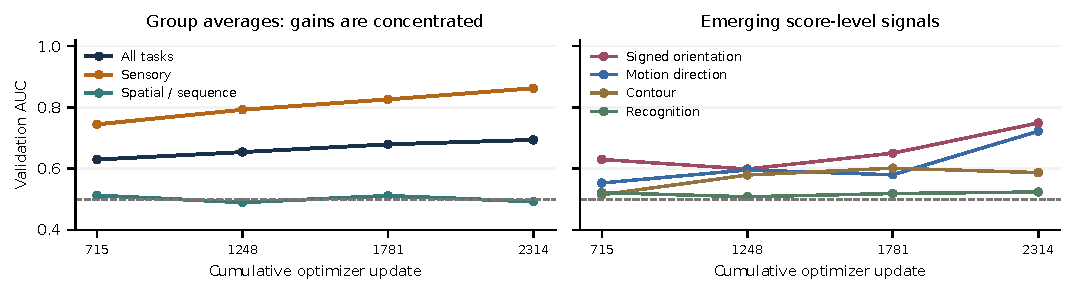
\includegraphics[width=1\linewidth,height=\textheight,keepaspectratio,alt={Saved validation snapshots only; dashed line is chance AUC. Group means are equal-task averages. No confidence intervals or newly generated model responses are implied.}]{validation_curves.pdf}
\caption{Saved validation snapshots only; dashed line is chance AUC.
Group means are equal-task averages. No confidence intervals or newly
generated model responses are implied.}
\end{figure}

\subsection{What these measurements do not
establish}\label{what-these-measurements-do-not-establish}

\textbf{No causal memory localization.} We have not shown that the
spatial matrices, rather than the GRU or frame stack, mediate successful
decisions in this joint learner. Architecture determines available
routes, not their behavioral use.

\textbf{No comparable reaction time.} Decisions are read at a prescribed
final frame. Wall-clock inference time, GRU confidence, an arbitrary
threshold crossing or an intermediate diagnostic head is not the paper's
learned wait/declare-change policy. An action-timing extension would be
a separate model/task experiment.

\textbf{No independent-source confidence interval.} New episode seeds do
not create new source photograph identities, and evaluation at trained
centers is not novel-location generalization. Per-task curves should
establish continued acquisition or a plateau before motivating
architecture changes. At weak baseline performance, interventions
chiefly test information use or vulnerability---not established
attentional benefits.

\newpage

\section{7. What Morgan, Albanna and Herman actually
manipulated}\label{what-morgan-albanna-and-herman-actually-manipulated}

The pinned reference is \emph{A recurrent vision transformer shows
signatures of primate visual attention}, arXiv:2502.10955v1 (2025). Its
recurrent ViT combines visual patches and activated memory to allocate
attention, updates patch-based LSTM memory, and uses an actor--critic
agent trained through reward. The task includes four Gabor locations,
probabilistic cue validity and a wait/declare-change action policy.
These are material differences from our end-of-trial supervised
classifiers.{[}1{]}

\subsection{Figure 5 is a computational allocation
intervention}\label{figure-5-is-a-computational-allocation-intervention}

Section 4.3 and Figure 5 describe artificially increasing bias toward a
spatial location, S1 or S4. The caption states that
\(\alpha_i(t_{\mathrm{change}})=1\) means the transmission
\(Z(t_{\mathrm{change}})\) is completely biased toward the corresponding
\(\xi_i(t_{\mathrm{change}})\). It reports response-rate and
reaction-time curves against orientation change, with 500 trials per
plotted data point.{[}1{]} This is the paper's computational analogue of
causal manipulation in attention-related primate circuitry. It is not a
literal model of electrode geometry, current amplitude or neural
recruitment.

The reference attention is source-normalized per query
(\(\sum_j\alpha_{ij}=1\); §6.5, Eqs. 7/14). Forcing one source to one
would zero the others \textbf{if that normalization is preserved}, but
Figure 5 does not specify the row/head overwrite or renormalization
algorithm. The direct sensory residual remains (Eqs. 8/15); this is not
erasure of all nonselected input.{[}1{]} Its spatial \(\alpha\) is not
our \textbf{per-key-row retention} \(\boldsymbol\alpha\).

\textbf{Read the legends by location, not colour.} Blue means
\(\alpha_1=1\) in A/B/D/E but \(\alpha_4=1\) in C/F. Bias toward the
changing location helps; bias toward the cued location does not
universally help. In C/F, the cue is at S1 and the change at S4: forcing
S1 impairs reporting, while forcing S4 improves it.{[}1{]}

Section 4.3 reports weaker cue-time effects and context-dependent
sensitivity/criterion effects.{[}1{]} These are textual claims here: the
pinned PDF refers to supplemental panels X/16 that it does not contain.
Exact clamp duration is also incompletely specified. We do not
reconstruct missing numerical results or infer that a different
recurrent architecture must share the timing effect.

\subsection{Comparability map}\label{comparability-map}

{\def\LTcaptype{none} % do not increment counter
\begin{longtable}[]{@{}
  >{\raggedright\arraybackslash}p{(\linewidth - 4\tabcolsep) * \real{0.3333}}
  >{\raggedright\arraybackslash}p{(\linewidth - 4\tabcolsep) * \real{0.3333}}
  >{\raggedright\arraybackslash}p{(\linewidth - 4\tabcolsep) * \real{0.3333}}@{}}
\toprule\noalign{}
\begin{minipage}[b]{\linewidth}\raggedright
Dimension
\end{minipage} & \begin{minipage}[b]{\linewidth}\raggedright
Reference recurrent ViT
\end{minipage} & \begin{minipage}[b]{\linewidth}\raggedright
Current joint KDA learner
\end{minipage} \\
\midrule\noalign{}
\endhead
\bottomrule\noalign{}
\endlastfoot
Manipulated substrate & Spatially biased transmission & Local state,
emission or feature drive \\
Memory organization & Patch-based LSTM with memory-guided attention &
Multi-resolution local associative fields plus global GRU \\
Task report & Detect any real orientation change & Task-specific signs,
target events, swaps, membership \\
Decision timing & Learned wait/declare-change policy & Fixed final-frame
classification \\
Cue manipulation & Explicit validity levels & Task-defining cues; no
matched validity series \\
Training & Sparse reward / actor--critic & Joint supervised
cross-entropy \\
Tested causal result & Artificial bias, behavioral timing and detection
& Not yet measured on this joint learner \\
\end{longtable}
}

The paper also reports that supervised variants could perform the task
without reproducing the same cueing effect.{[}1{]} Consequently, even
eventual high accuracy on our suite would not by itself predict
primate-like attention dynamics. Functional comparability requires
matched behavioral questions and controls, not merely recurrent state
and a spatial mask.

\newpage

\section{8. A concrete computational microstimulation
protocol}\label{a-concrete-computational-microstimulation-protocol}

\textbf{Proposed only.} Freeze a preselected trained checkpoint and all
model weights. Replay identical existing-task episodes under sham and
intervention, preserving input rasters, labels, trial order and RNG. An
analysis wrapper may use actual renderer phase indices to apply a pulse;
those indices must not enter the deployed model or become a learned
gate. First verify the unmodified wrapper against the ordinary forward
path within a stated numerical tolerance.

\subsection{Primary intervention: perturb the local emitted
representation}\label{primary-intervention-perturb-the-local-emitted-representation}

At one scale, after KDA's output projection and before concatenation,
apply\\
\[
\widetilde O_t(p)=O_t(p)+\lambda\,g(t)\,m_s(p)\,\sigma_s\,d_s.
\]\\
Start at the \(13\times13\) scale. Here \(m_s(p)\) is a scene-centred
Gaussian mask with saved radius and unit peak; \(g(t)\) specifies
onset/duration; \(d_s\) is a unit-norm 32-channel direction. Set
\(\sigma_s^2=\mathbb E_{\rm cal}\|O-\mu_{\rm cal}\|_2^2\), estimated at
the declared task/epoch on independent calibration trials. Save achieved
perturbation norms; equal peak doses do not imply equal total dose
across mask sizes. Dose \(\lambda\) is dimensionless, not microamperes.

Calibrate a task-relevant direction independently of final evaluation:
for example, a signed feature contrast from matched calibration trials,
or a prespecified projection of a fitted calibration decoder. Validate
the direction on a separate split. Include equal-norm random or
orthogonal patterns and both signs where meaningful. Adding a positive
constant to every signed channel is not an identified physiological
excitation. Initial exploratory doses such as \(0,\pm0.25,\pm0.5,\pm1\)
are \textbf{proposed relative scales}, not known safe or effective
operating points.

This intervention changes what downstream processing receives at that
timestep. It does not directly overwrite the same module's state. It can
nevertheless change higher-scale memory and the GRU, creating lasting
behavioral consequences. Persistence after an emission pulse must not be
misreported as proof that the directly stimulated local matrix was
modified.

\subsection{Secondary intervention: persistently perturb the
association}\label{secondary-intervention-persistently-perturb-the-association}

To distinguish stored-content effects, perturb the updated state before
readout:\\
\[
\widetilde S_t(p,h)=S_t(p,h)
  +\lambda\,g(t)\,m_s(p)\,\sigma_{S,s,h}\,a_h b_h^\top,
\]\\
with calibrated unit vectors \(a_h\in\mathbb R^8\),
\(b_h\in\mathbb R^{16}\). Specify one or both heads. The perturbed
matrix must produce the current readout \textbf{and be carried forward}.
Before output projection, its immediate effect is
\(\Delta o=\lambda g m\sigma_S(a_h^\top q_t)b_h\): even a large state
pulse can be invisible to an orthogonal query. A readout-only copy
instead tests transient access. This perturbs associative content, not
isolated attention allocation or identified biological synapses.

\subsection{Controls and closer---but nonidentical---allocation
analogues}\label{controls-and-closerbut-nonidenticalallocation-analogues}

A local emission gain, \(\widetilde O=(1+\lambda g m)O\), changes
existing influence without adding a new pattern. A norm-matched
suppression toward a stated reference tests a complementary direction.
Neither creates the reference ViT's competitive spatial allocation:
increasing one site does not automatically remove other sites'
contributions. A renormalized routing operator could impose that
competition, but it would be a new diagnostic computation, not an
existing KDA control variable or an exact replication. Do not silently
substitute it for a state or emission intervention.

Log substrate, scale, head, site mask, epoch, dose, achieved
feature/state change and downstream propagation. Start with one declared
scale and substrate rather than a broad search for an attractive result;
confirmatory doses/sites must be fixed before their final evaluation.

\newpage

\section{9. Experimental design and behavioral
readouts}\label{experimental-design-and-behavioral-readouts}

A meaningful microstimulation study compares \textbf{where},
\textbf{when} and \textbf{what} was perturbed while holding physical
evidence fixed. Use paired episodes, not unrelated stimulus draws, for
sham-versus-pulse contrasts. Save per-trial responses and the actual
spatial arrays; region averages cannot reconstruct per-timestep maps. No
extraction or intervention run is authorized by this document.

\subsection{Site × epoch × dose design}\label{site-epoch-dose-design}

Compare the cued/queried site, a matched uncued site and an off-target
control. For retrospective binding, the queried location is not known
from an encoding cue; distinguish that analysis label from information
available to the model. Match masks by scene-space geometry and disclose
unequal feature coverage across resolutions. Spatially localized
injection can have distributed consequences through convolutions and
GroupNorm.

Separate cue presentation, sample encoding, early nominal blanks,
genuinely stimulus-free retention and probe/change/report. The
three-frame stack carries samples into the first two blanks, so use
actual input-stack contents to verify blank eligibility. Cue pulses may
be duplicated through the raw input stack if applied to images, whereas
a one-step internal emission pulse is a different intervention. Declare
the timing convention explicitly. Use trial-relative discrete frames
unless a renderer supplies physical timing; do not equate all task
frames with the Krauzlis 100 Hz clock.

\subsection{Psychometrics before aggregate
accuracy}\label{psychometrics-before-aggregate-accuracy}

For orientation, plot positive-report probability against \textbf{signed
target change}, conditioning on foil changes, cue meaning, stimulated
site and dose. For the ring task, the label is rotation sign; for signed
cued orientation, it is agreement with the instructed sign, with
unchanged negatives. A positive response at zero change has different
semantics in those tasks. Do not mechanically fit the reference paper's
change-detection psychometric function to a different report rule.

For Krauzlis, plot target hit rate, foil-event positive rate and catch
positive rate separately. For binding, a foil-only exchange is the
negative condition, not a no-change image. Recognition requires nonempty
membership sensitivity plus separate empty-set specificity.
Motion-duration effects should be stratified by count-winner margin and
recent motion history where the native metadata permits, rather than
assuming a change-detection interpretation.

Where binary signal/noise classes are meaningful, estimate\\
\[
 d'=\Phi^{-1}(H)-\Phi^{-1}(F),\qquad
 c=-\tfrac12[\Phi^{-1}(H)+\Phi^{-1}(F)].
\]\\
Define \(H\) and \(F\) for each task; analyze Krauzlis catch and foil
comparisons separately rather than silently pooling them. Correct rates
of zero or one with a declared finite-sample rule, for example
\((k+0.5)/(n+1)\). For four-choice tasks use the confusion matrix and
class-specific effects, not an unexplained binary \(d'\). Criterion
shifts alone can change response rates without enhancing discrimination.

\subsection{Uncertainty, specificity and
falsification}\label{uncertainty-specificity-and-falsification}

Estimate within-episode sham/pulse differences with paired resampling;
keep multiple doses, delays or repetitions of the same base episode
grouped. Photograph-based uncertainty should account for reused source
identities. Independent trained seeds address a different uncertainty
than more trials from one model. Fix primary comparisons in advance and
label secondary site/epoch searches exploratory.

A selective site-by-epoch interaction, a graded dose relation and
task-appropriate psychometric shifts would support a functional effect.
Uniform degradation at all sites, positive-report increases with equal
false-alarm increases, or effects duplicated by random patterns favor
nonspecific disruption or response bias. A null effect can reflect
ineffective stimulation, saturation, redundant pathways or poor baseline
competence; verify the achieved manipulation before concluding that a
region is unnecessary.

\newpage

\section{10. Expected outcomes, comparability and next
decisions}\label{expected-outcomes-comparability-and-next-decisions}

\textbf{Are the experiments comparable?} At the level of a causal
question---does increasing the influence of a spatial representation
change perception in a site- and time-specific manner?---yes. At the
level of manipulated variable, task, action policy and biological
implementation, not directly. A rigorous study should report which
levels were matched rather than collapse them into a yes/no equivalence
claim.

\textbf{Do we expect the same results?} Not as a default. The
reference's change-time effect and weak cue-time effect motivate
directional hypotheses.{[}1{]} Our cue encoding, temporal stacking,
local associative state and supervised decision rule could produce
strong encoding effects, persistent storage distortions, immediate
report bias, compensatory processing or no measurable benefit. The
present weak spatial competence makes a clean attentional-enhancement
prediction especially premature.

{\def\LTcaptype{none} % do not increment counter
\begin{longtable}[]{@{}
  >{\raggedright\arraybackslash}p{(\linewidth - 4\tabcolsep) * \real{0.3333}}
  >{\raggedright\arraybackslash}p{(\linewidth - 4\tabcolsep) * \real{0.3333}}
  >{\raggedright\arraybackslash}p{(\linewidth - 4\tabcolsep) * \real{0.3333}}@{}}
\toprule\noalign{}
\begin{minipage}[b]{\linewidth}\raggedright
Observation in a future study
\end{minipage} & \begin{minipage}[b]{\linewidth}\raggedright
Supported interpretation
\end{minipage} & \begin{minipage}[b]{\linewidth}\raggedright
Not established
\end{minipage} \\
\midrule\noalign{}
\endhead
\bottomrule\noalign{}
\endlastfoot
Stimulated-site sensitivity rises with stable false alarms & Selective
improvement under that intervention & Same circuit as FEF/SC or
identical ViT mechanism \\
Hits and false alarms rise together & Response-bias component & Improved
sensory information \\
Local state pulse persists across true blanks & Perturbed recurrent
route affects later behavior & All memory resides at that site \\
Emission pulse changes behavior but state pulse does not &
Substrate-dependent causal access at tested doses & Stored information
is absent \\
Cue pulse differs from probe pulse & Temporal specificity & Replication
unless task/timing are matched \\
All interventions cause broad degradation & Possible nonspecific
disruption & Attention-specific causal mechanism \\
\end{longtable}
}

\textbf{Decision sequence.} Finish the authorized training and inspect
per-task acquisition. Select the checkpoint without stimulation-test
outcomes. Establish the relevant baseline psychometrics, separate
calibration/selection/test episodes, verify sham equivalence, and only
then run one bounded intervention family. If the existing task cannot
support a valid-neutral comparison or genuine response timing, label
those outcomes unavailable; implementing the reference task or a timed
action policy would require a separately authorized experiment. Do not
change teaching or architecture merely to obtain the anticipated effect.

\textbf{Biological anchor.} Cavanaugh, Alvarez and Wurtz stimulated
superior colliculus around a possible dot-motion change: 600 ms
beginning 150 ms before the first motion epoch ended (Fig. 2A). Hits
generally increased while false positives changed little, motivating
explicit false-report controls rather than hits alone.{[}2{]} That
electrical intervention recruits biological circuitry; neither a ViT
allocation clamp nor a KDA feature pulse has a validated conversion to
its current, tissue extent or temporal scale.

\subsection{Reproducibility and source
map}\label{reproducibility-and-source-map}

\textbf{{[}C1{]}} \texttt{WorkingMemory/PlainBaseline/accum.py:40–75}:
convolutional hierarchy, stack, projection, GRU and heads.
\textbf{{[}C2{]}}
\texttt{PreAttentiveVision/TemporalIntegration/accumulators.py:19–66}:
exact KDA update and gates. \textbf{{[}C3{]}}
\texttt{SecondPass/TaskSuite/\{README.md,catalog.json,suite.py\}}: task
laws, streams and reporting. \textbf{{[}C4{]}}
\texttt{SecondPass/JointTraining/\{worker.py,core.py,continuation\_v3.py,AMENDMENT\_V3.md\}}:
optimizer, selection and continuation contract.

\textbf{{[}R1{]}}
\texttt{SecondPass/JointTraining/runs/fresh\_kda\_joint\_01\_continuation\_v2/}:
\texttt{report.json}, \texttt{test\_terminal.json},
\texttt{test\_selected.json}. Terminal checkpoint 715 was used for the
completed-test column, not historical winner 117. \textbf{{[}R2{]}}
\texttt{.../fresh\_kda\_joint\_01\_continuation\_v3\_8h/}: scheduled
validation JSONs and \texttt{progress.jsonl}. Snapshot files and
figure-building scripts are retained beside this report. Historical
orientation-lineage interventions are not evidence for this joint model.

\textbf{{[}R3{]}} Beside this report: \texttt{metrics\_snapshot.json},
\texttt{architecture\_metrics\_notes.md},
\texttt{paper\_comparison\_notes.md} and
\texttt{paper\_evidence/verified\_quotes.json}. The audit verifies six
complete 13-task/35-cell evaluations, parameter counts, checkpoint
shapes and source digests without model inference.

\subsection{Sources}\label{sources}

{[}1{]} https://arxiv.org/html/2502.10955v1 --- Morgan, Albanna and
Herman (2025), A recurrent vision transformer shows signatures of
primate visual attention, pinned v1\\
{[}2{]} https://www.jneurosci.org/content/26/44/11347 --- Cavanaugh,
Alvarez and Wurtz (2006), Enhanced Performance with Brain Stimulation:
Attentional Shift or Visual Cue?, Journal of Neuroscience
26:11347--11358

\end{document}
